% $Header: /cvsroot/latex-beamer/latex-beamer/solutions/conference-talks/conference-ornate-20min.en.tex,v 1.6 2004/10/07 20:53:08 tantau Exp $

\documentclass{beamer}

\mode<presentation>
{
  \usetheme{Hawke}
  % or ...

  \setbeamercovered{transparent}
  % or whatever (possibly just delete it)
}


\usepackage[english]{babel}
% or whatever

\usepackage[latin1]{inputenc}
% or whatever

\usepackage{times}
\usepackage[T1]{fontenc}

\usepackage{multimedia}


%%%%%%
% My Commands
%%%%%%

\newcommand{\bb}{{\boldsymbol{b}}}
\newcommand{\bx}{{\boldsymbol{x}}}
\newcommand{\by}{{\boldsymbol{y}}}
\newcommand{\bfm}[1]{{\boldsymbol{#1}}}

%%%%

\title[Lecture 17] % (optional, use only with long paper titles)
{Lecture 17 - Predictor Corrector Methods}


\author[I. Hawke] % (optional, use only with lots of authors)
{I.~Hawke}

\institute[University of Southampton] % (optional, but mostly needed)
{
%  \inst{1}%
  School of Mathematics, \\
  University of Southampton, UK
}

\date[Semester 1] % (optional, should be abbreviation of conference name)
{MATH3018/6141, Semester 1}

\subject{Numerical methods}
% This is only inserted into the PDF information catalog. Can be left
% out.


\pgfdeclareimage[height=0.5cm]{university-logo}{mathematics_7469}
\logo{\pgfuseimage{university-logo}}


\AtBeginSection[]
{
  \begin{frame}<beamer>
    \frametitle{Outline}
    \tableofcontents[currentsection]
  \end{frame}
}



\begin{document}

\begin{frame}
  \titlepage
\end{frame}

\section{Predictor-Corrector methods}

\subsection{Predictor-Corrector methods}

\begin{frame}
  \frametitle{Geometrical interpretation of Euler's method}

  Considering IVPs in the form
  \begin{equation*}
    \by'(x) = \bfm{f}(x, \by(x)).
  \end{equation*}

  The simple (first order accurate, explicit) Euler method is
  \begin{equation*}
    \by_{n+1} = \by_n + h \bfm{f}(x_n, \by_n).
  \end{equation*} \pause

  Euler's method is not sufficiently accurate for practical use. Euler predictor-corector is second order. \pause

  Use \emph{multiple} approximations to the slope for a more accurate result.

\end{frame}


\section{Runge-Kutta methods}

\subsection{Runge-Kutta methods}

\begin{frame}
  \frametitle{Runge-Kutta methods}

  In a Runge-Kutta method, Taylor's theorem is used from the start to
  ensure the desired accuracy. \pause

  \vspace{1ex}

  Consider a single step from known data $y_n(x_n)$. Compute one
  estimate ($k_1$) for $f(x_n, y_n)$ using the known data. \pause Then
  compute $y^{(1)}$ at $x_n + \alpha h$ using $y_n + \beta k_1$. \pause
  From this compute another estimate ($k_2$) for $f(x, y)$ at
  $x_n + \alpha h$. Compute $y^{(2)}$ etc; combine as $y_{n+1} = a k_1 + b k_2 + \dots$. \pause

  \vspace{1ex}

  Such methods are called \emph{multistage}:
  \begin{itemize}
  \item a number of estimates of $f$ are combined to
    improve accuracy;
  \item only the previous value $y_n$ is required to start the
    algorithm.
  \end{itemize}

  \vspace{1ex}

  To derive $a, b, \dots, \alpha, \beta, \dots$ expand the algorithm and match to
  exact solution using Taylor's theorem, chain rule and IVP.

\end{frame}

\begin{frame}
  \frametitle{Example: RK2}

  \begin{overlayarea}{\textwidth}{0.8\textheight}
    \only<1|handout:1>
    {
      For the second order method we have
      \begin{align*}
        y_{n+1} & = y_n + a k_1 + b k_2, \\
        k_1 & = h f(x_n, y_n), \\
        k_2 & = h f(x_n + \alpha h, y_n + \beta k_1).
      \end{align*}
      We have four free parameters $a, b, \alpha, \beta$ to fix.
    }
    \only<2|handout:1>
    {
      Taylor expand the definition of $y_{n+1} = y(x_n + h)$:
      \begin{align*}
        y_{n+1} & = y_n + h y'_n + \tfrac{h^2}{2} y''_n + \dots \\
        & = y_n + h f_n +  \tfrac{h^2}{2} \left( f_n \right)' + \dots \\
        \intertext{using the original IVP, then use the chain rule:}
        & = y_n + h f_n +  \tfrac{h^2}{2} \left( \partial_x f_n +
          (\partial_y f)_n f_n \right) + \dots .
      \end{align*}
    }
    \only<3-|handout:2>
    {
      Algorithm:
      \begin{align*}
        y_{n+1} & = y_n + a k_1 + b k_2 \\
        & = y_n + h f_n +  \tfrac{h^2}{2} \left( \partial_x f_n +
          (\partial_y f)_n f_n \right) + \dots
      \end{align*}

      Compare against the Taylor expansion of the second order
      method
      \begin{align*}
        y_{n+1} & = y_n + a h f_n + b h f(x_n + \alpha h, y_n + \beta h
        f_n) \\
        & = y_n + h (a + b) f_n + h^2 \left[ (\partial_x f)_n \alpha b +
          (\partial_y f)_n f_n \beta b \right].
      \end{align*}
    }
    \only<4|handout:2>
    {
      Matching coefficients
      \begin{equation*}
        \left\{
          \begin{aligned}
            a + b & = 1 \\
            \alpha b & = 1 / 2 \\
            \beta b & = 1 / 2
          \end{aligned}
          \right. .
      \end{equation*}
    }
  \end{overlayarea}

\end{frame}

\begin{frame}
  \frametitle{Example: RK2 (II)}

  The RK2 method
  \begin{align*}
    y_{n+1} & = y_n + a k_1 + b k_2, \\
    k_1 & = h f(x_n, y_n), \\
    k_2 & = h f(x_n + \alpha h, y_n + \beta k_1)
  \end{align*}
  with coefficients
  \begin{equation*}
    \left\{
      \begin{aligned}
        a + b & = 1 \\
        \alpha b & = 1 / 2 \\
        \beta b & = 1 / 2
      \end{aligned}
    \right.
  \end{equation*}
  is not completely specified; there is essentially one free
  parameter. \pause

  \vspace{1ex}

  Not all choices are stable. The classic choice is $a = 1/2 = b$,
  $\alpha = 1 = \beta$: this is Euler predictor-corrector.

\end{frame}

\begin{frame}
  \frametitle{Runge-Kutta 4}

  The most used is the classic fourth order Runge-Kutta method. This
  requires fixing eight free parameters by matching to order
  $h^4$. This gives a family of methods again. \pause

  \vspace{1ex}

  Standard choice is
  \begin{align*}
    y_{n+1} & = y_n + \tfrac{1}{6} \left( k_1 + 2 (k_2 + k_3) + k_4
    \right), \\
    k_1 & = h f(x_n, y_n), \\
    k_2 & = h f(x_n + h / 2, y_n + k_1 / 2), \\
    k_3 & = h f(x_n + h / 2, y_n + k_2 / 2), \\
    k_4 & = h f(x_n + h    , y_n + k_3    ).
  \end{align*} \pause

  \vspace{1ex}

  The local error term is ${\cal O}(h^5)$ leading to a global error
  ${\cal O}(h^4)$.

\end{frame}


\begin{frame}
  \frametitle{Example}


  Apply the RK4 method to
  \begin{equation*}
    y'(x) = - \sin(x), \quad y(0) = 1.
  \end{equation*}
  Integrate to $x = 0.5$. Using $h = 0.1$ gives an error $4.8 \times
  10^{-7}\%$; using $h = 0.01$ gives an error of $4.8 \times
  10^{-11}\%$, showing fourth order convergence. \pause

  \vspace{1ex}

  Compare with an error, for $h=0.01$, of $10^{-3}\%$ for the Euler
  predictor-corrector method, and $0.24\%$ for the simple Euler
  method.

  \vspace{1ex}

  RK4 more efficient \emph{despite} needing four times the function
  evaluations of Euler's method.

\end{frame}


\begin{frame}
  \frametitle{Example: 2}


  Consider the system
  \begin{equation*}
    \left\{
      \begin{aligned}
        \dot{x} & = -y \\ \dot{y} & = x
      \end{aligned} \right., \quad x(0) = 1, \, \, y(0) = 0.
  \end{equation*}
  In polar coordinates this is $\dot{r} = 0$, $\dot{\phi} = 1$.
  \begin{columns}
    \begin{column}{0.5\textwidth}
      \begin{overlayarea}{\textwidth}{0.4\textheight}
        \only<2-3|handout:1>
        {
          Use the RK4 method with $h=0.1$. At $t=500$ the
          result matches the correct answer to the eye.
        }
        \only<3|handout:1>
        {

          \vspace{1ex}
          The growth of the radius makes the errors visible, but they
          are still tiny.

        }
        \only<4-5|handout:2>
        {
          Use the RK4 method with $h=0.01$. At $t=500$
          the result matches the correct answer to the eye.
        }
        \only<5|handout:2>
        {

          \vspace{1ex}
          The growth of the radius remains, but is minute.
        }
      \end{overlayarea}
    \end{column}
    \begin{column}{0.5\textwidth}
      \begin{overlayarea}{\textwidth}{0.6\textheight}
        \only<2|handout:0>
        {
          \begin{center}
            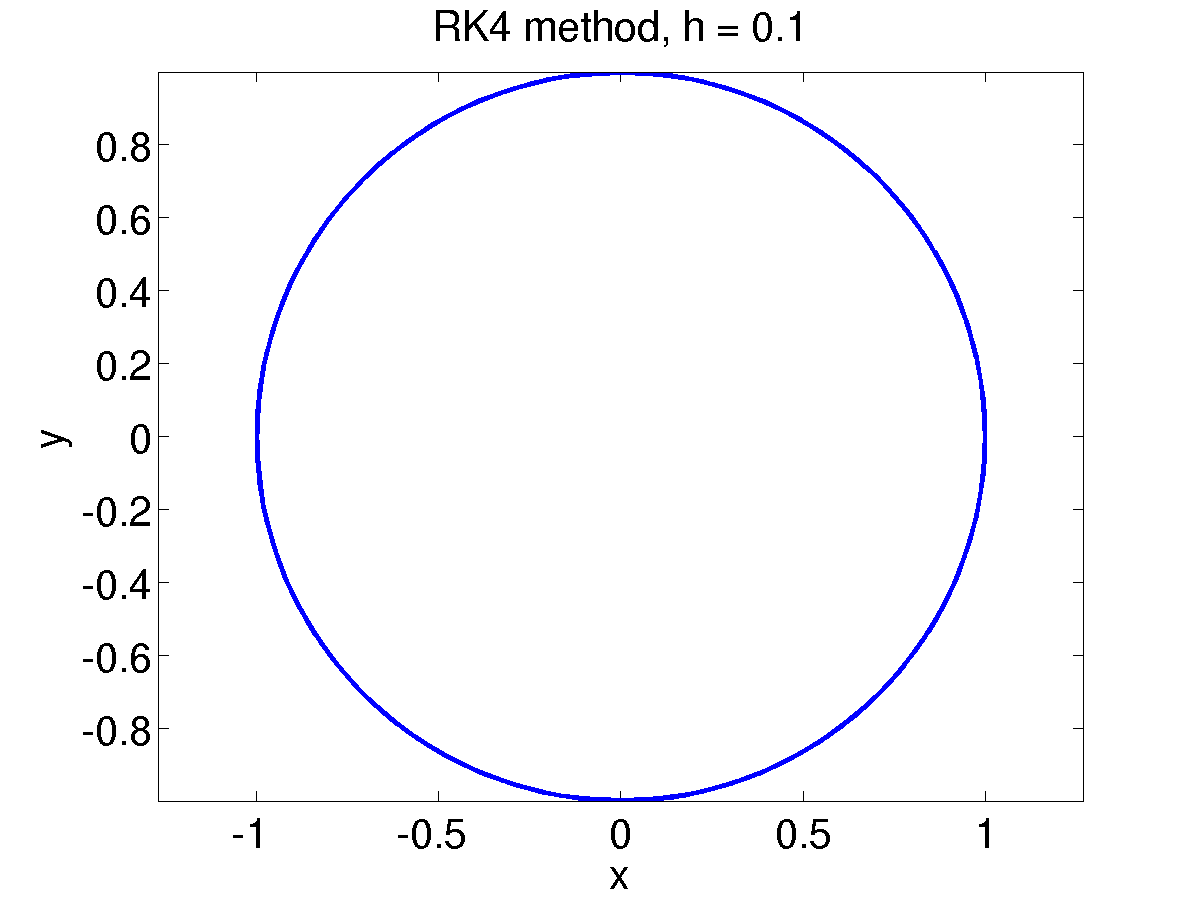
\includegraphics[height=0.5\textheight]{figures/RK4_1}
          \end{center}
        }
        \only<3|handout:1>
        {
          \begin{center}
            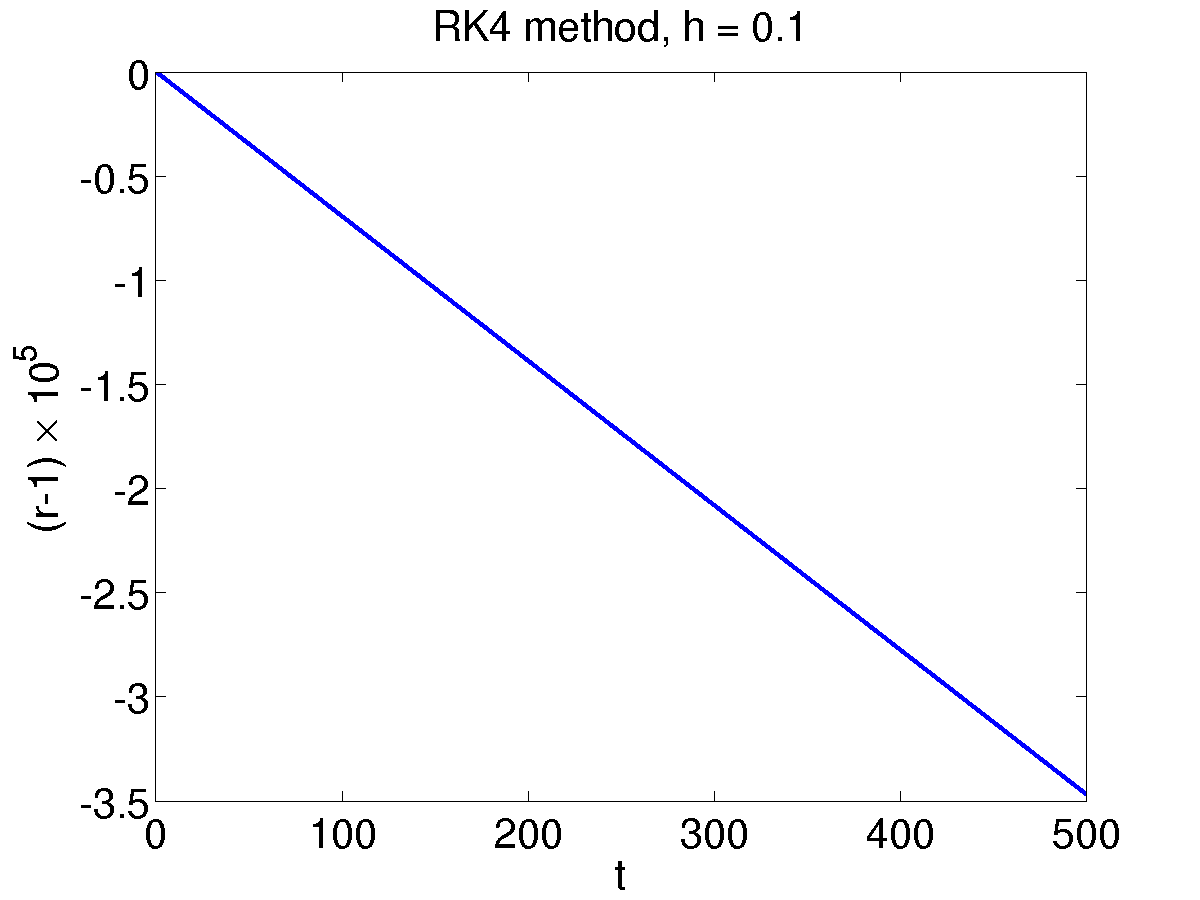
\includegraphics[height=0.5\textheight]{figures/RK4_rad1}
          \end{center}
        }
        \only<4|handout:0>
        {
          \begin{center}
            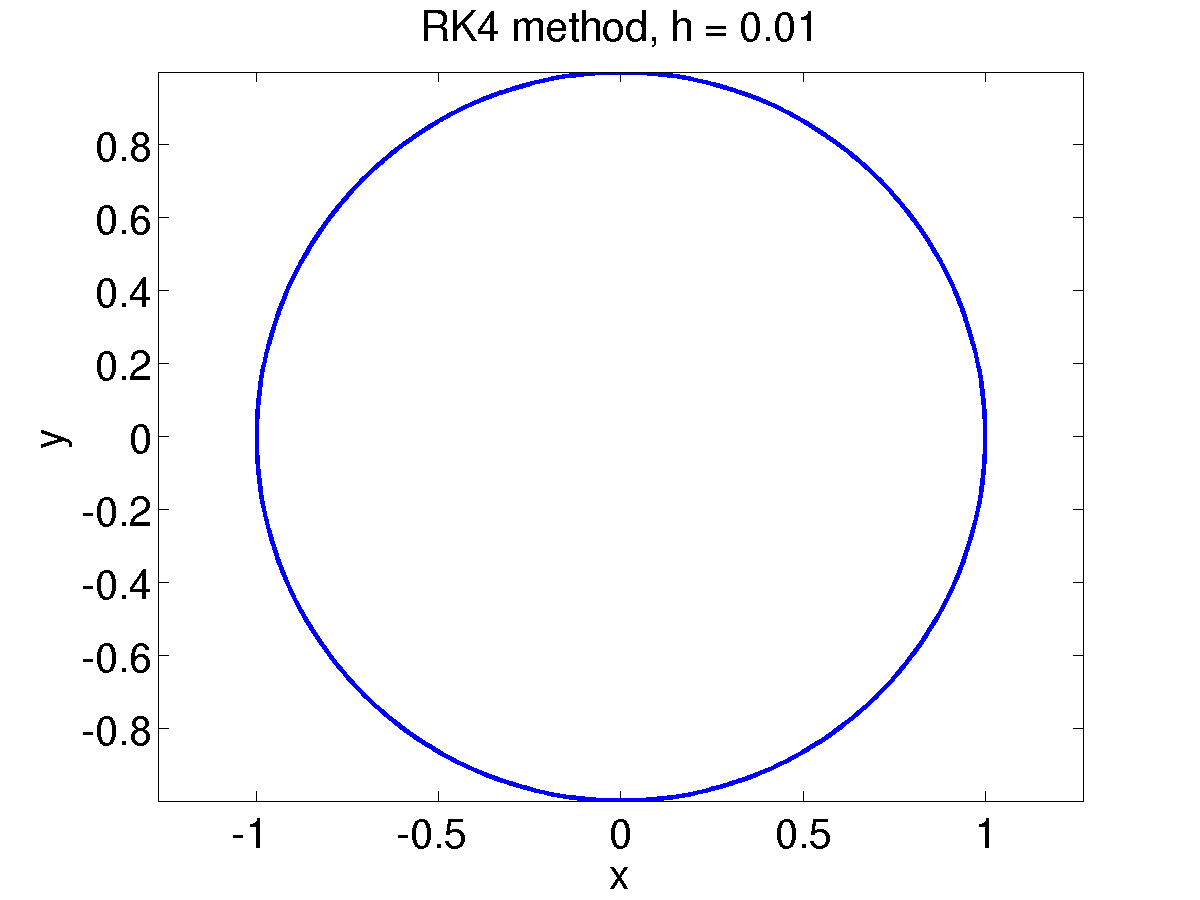
\includegraphics[height=0.5\textheight]{figures/RK4_2}
          \end{center}
        }
        \only<5|handout:2>
        {
          \begin{center}
            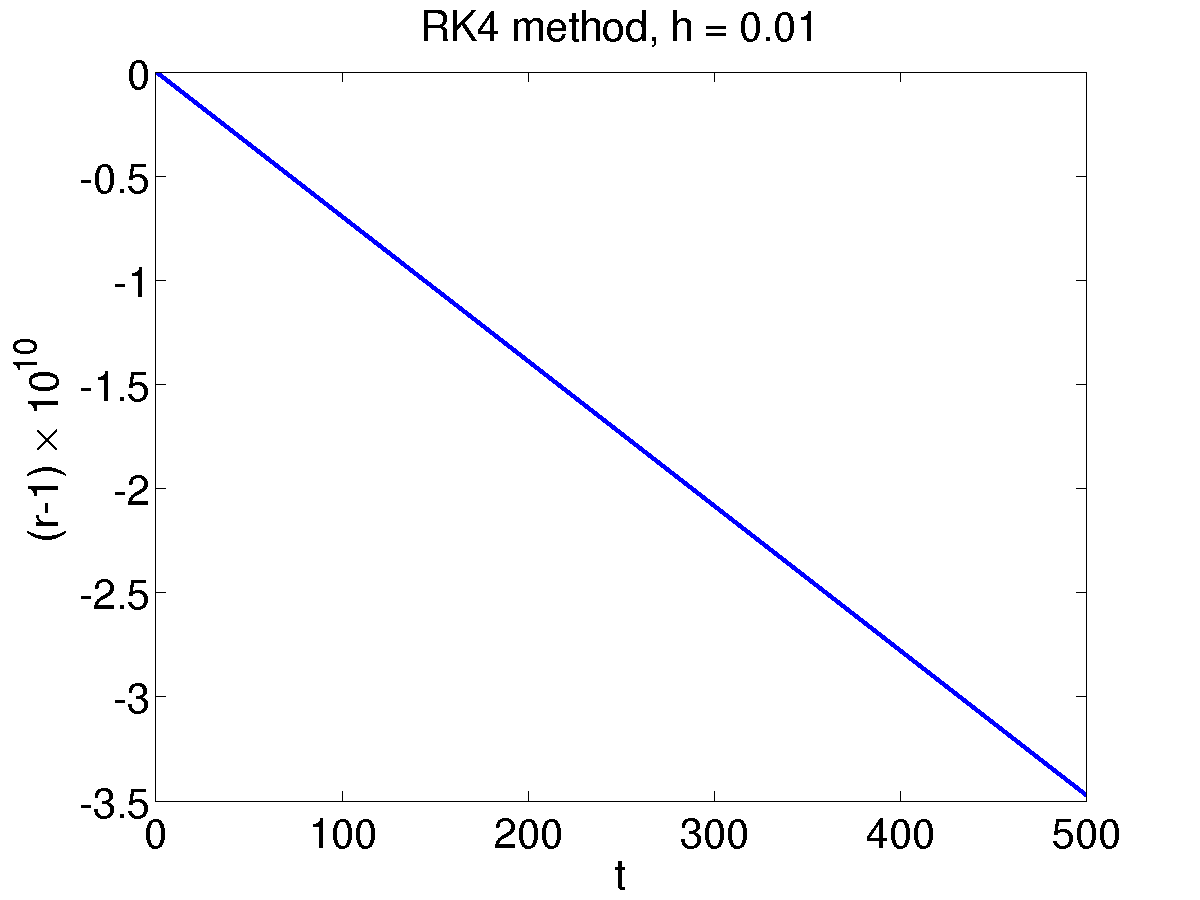
\includegraphics[height=0.5\textheight]{figures/RK4_rad2}
          \end{center}
        }
      \end{overlayarea}
    \end{column}
  \end{columns}

\end{frame}


\section{Summary}

\subsection{Summary}

\begin{frame}
  \frametitle{Summary}

  \begin{itemize}
  \item Euler's method has local error $\propto h^2$, hence global
    error $\propto h$.
  \item The Euler predictor-corrector method has local error $\propto
    h^3$, hence global error $\propto h^2$.
  \item \emph{Multistage} methods such as Runge-Kutta methods require
    only one known value $\by_{n}$ to start, and compute (many)
    estimates of the function $\bfm{f}$ for the algorithm to update
    $\by_{n+1}$.
  \item Runge-Kutta methods are the classic multistage methods; the
    predictor-corrector method is a second order RK method.
  \item RK4 is useful in practice.
  \end{itemize}

\end{frame}

\end{document}
